%*----------- SLIDE (IMAGEM DO PROJETO) -------------------------------------------------------------
 \begin{frame}[c]{APEREA}
    \begin{figure}
        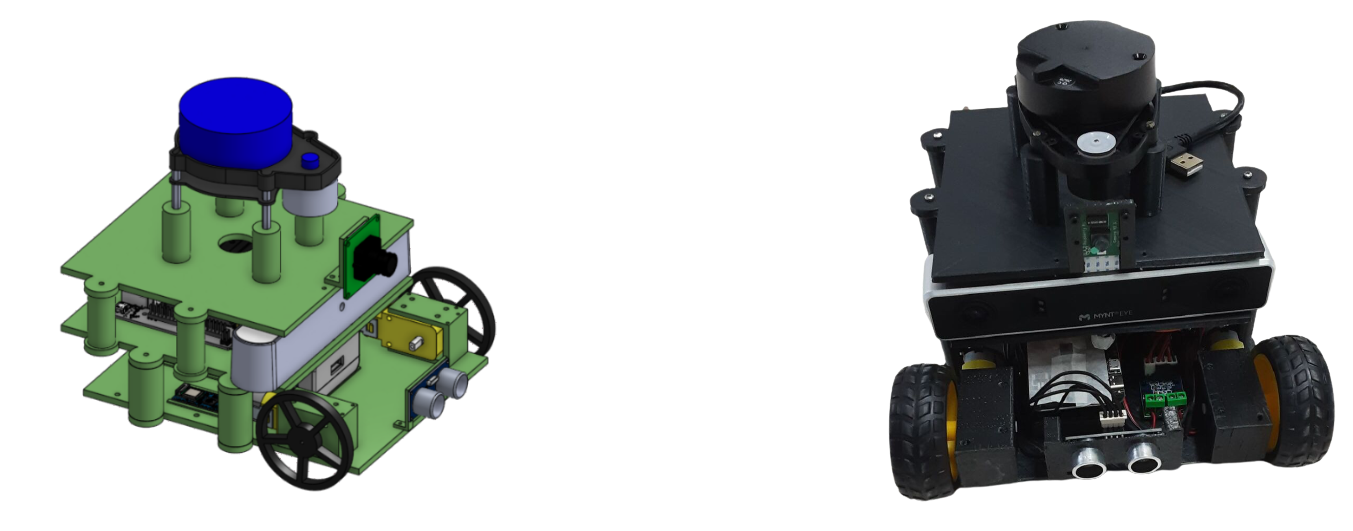
\includegraphics[width=\textwidth]{1-aperea.png}
        %\caption{.}
    \end{figure}
\end{frame}

%*----------- SLIDE -------------------------------------------------------------
\begin{frame}[t]{Conceitual}
    \framesubtitle{Objetivo}
    
    O Aperea é capaz de \emph{buscar} e \emph{reconhecer} uma \emph{tag} no ambiente. A tag indica a localização de uma bola na cor laranja. A partir desta informação, o robô deve \emph{encontrar} a \emph{bola}.

    \vspace*{0.8cm}
    \begin{figure}
        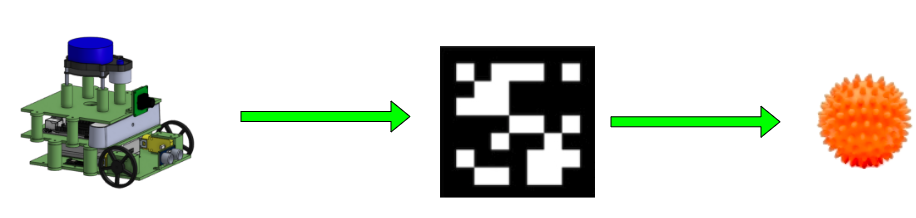
\includegraphics[trim = 0 20 0 50, clip, width=0.8\textwidth]{jetbot_mission.png}
        %\caption{.}
    \end{figure}
%*----------- notes
    \note[item]{Notes can help you to remember important information. Turn on the notes option.}
\end{frame}
%-

%*----------- SLIDE -------------------------------------------------------------
\begin{frame}[t]{Conceitual} 
    \framesubtitle{Requisitos do projeto}
        \begin{columns}[t]
            \column{.05\linewidth}
            \column{.4\linewidth}
                \begin{enumerate}
                    \item O robô deve ser autônomo
                    \item O robô deve mapear e reconhecer o ambiente
                    \item O robô deve ser capaz de evitar obstáculos
                    \item O robô deve reconhecer uma esfera colorida
                \end{enumerate}
            \column{.6\linewidth}
            \begin{center}
            %\centerline{
                \begin{figure}
                    \roundpic[xshift=-0.7cm,yshift=0.5cm]{6cm}{6cm}{aperea_assembly2}
                \end{figure}
            %}
            \end{center}
        \end{columns}
%*----------- notes
    \note[item]{Notes can help you to remember important information. Turn on the notes option.}
\end{frame}
%-
%*----------- SLIDE (IMAGEM DO PROJETO) -------------------------------------------------------------
\begin{frame}[t]{Conceitual}
    \framesubtitle{Metodologia}
    \begin{figure}
        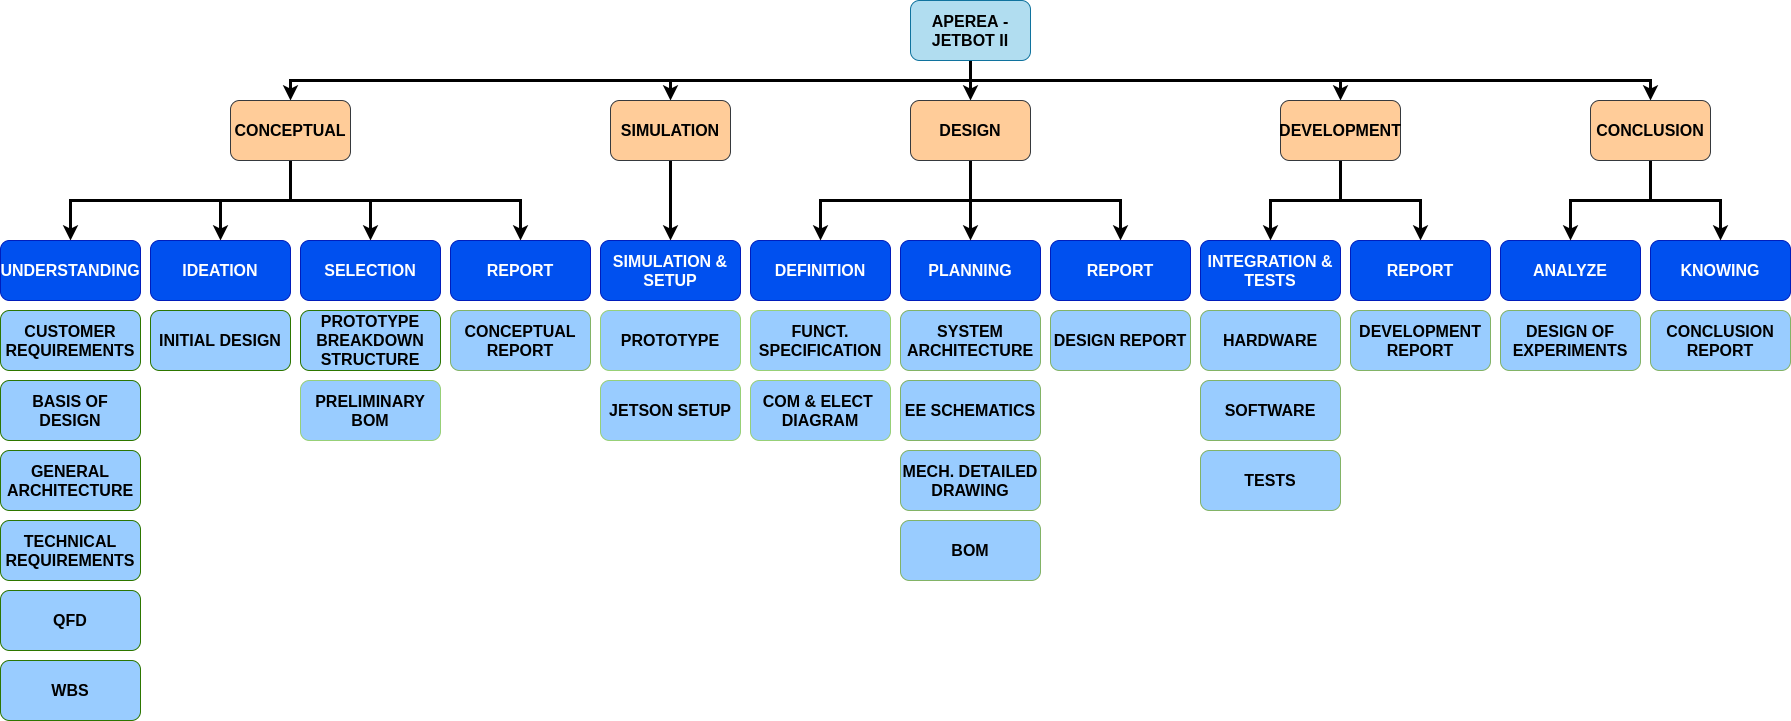
\includegraphics[width=0.8\textwidth]{eap.png}
        %\caption{.}
    \end{figure}
\end{frame}
%*----------- SLIDE (IMAGEM DO PROJETO) -------------------------------------------------------------
\begin{frame}[t]{Design}
    \framesubtitle{Linha do tempo do design}
    \begin{figure}
        % 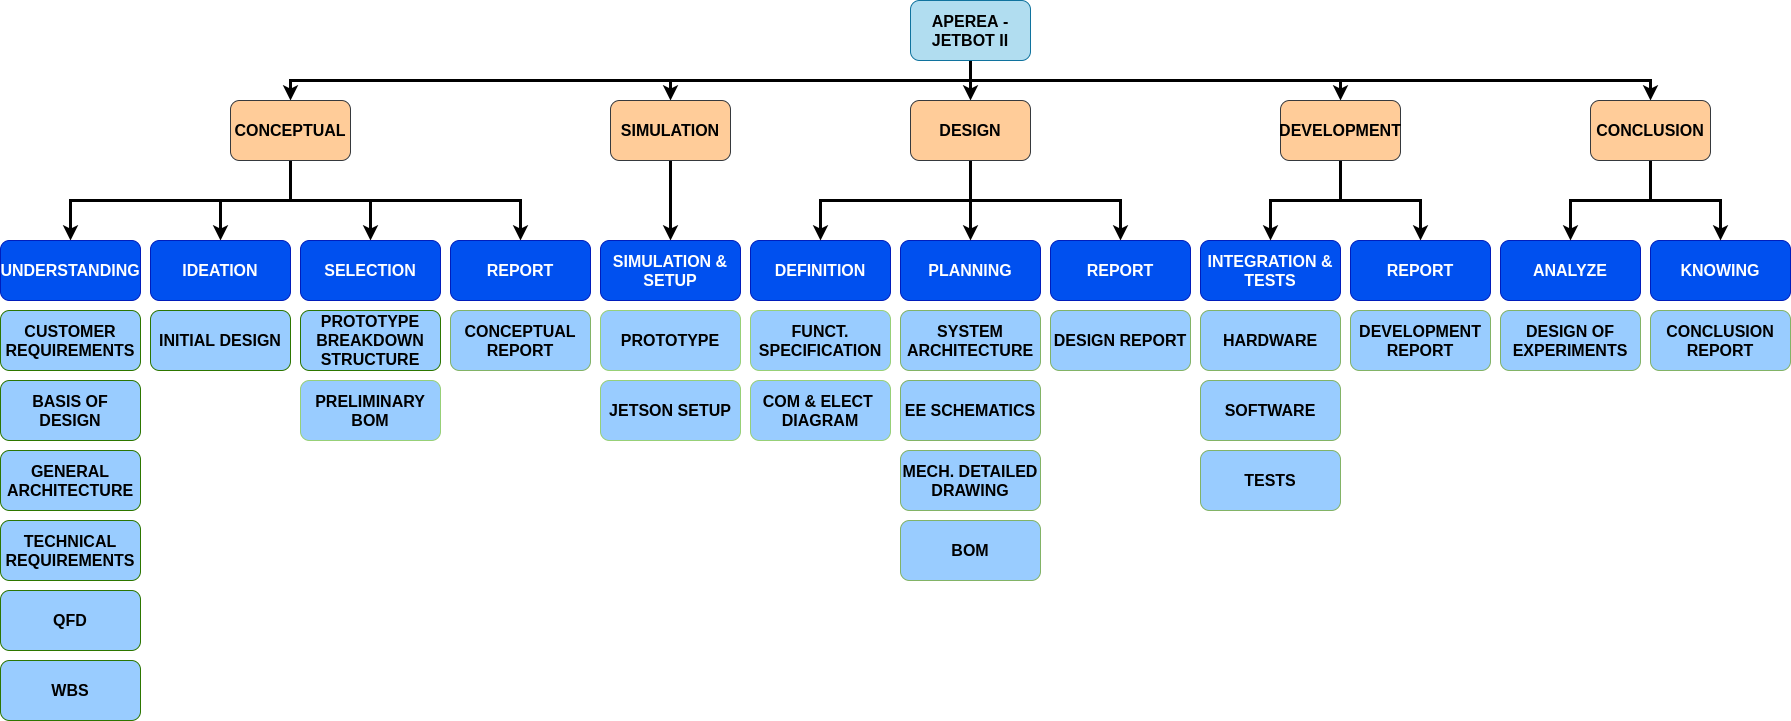
\includegraphics[width=\textwidth]{eap.png}
        %\caption{.}
    \end{figure}
\end{frame}

%*----------- SLIDE (IMAGEM DO PROJETO) -------------------------------------------------------------
\begin{frame}[t]{Design}
    \framesubtitle{Arquitetura Geral}
    \begin{figure}
        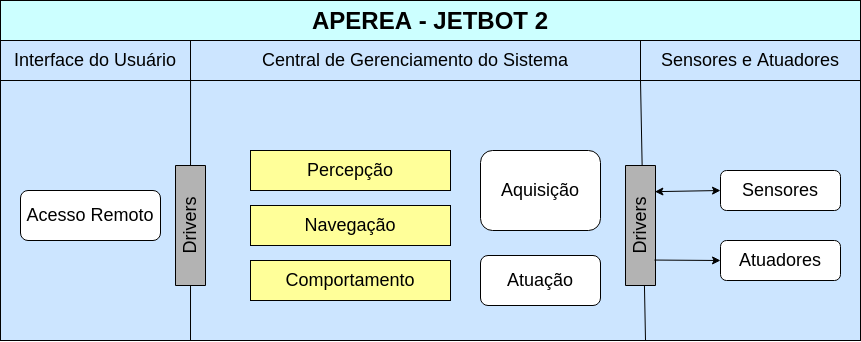
\includegraphics[width=\textwidth]{AG.png}
        %\caption{.}
    \end{figure}
\end{frame}

%*----------- SLIDE (IMAGEM DO PROJETO) -------------------------------------------------------------
\begin{frame}[t]{Design}
    \framesubtitle{Funcionalidades}
    \begin{figure}
        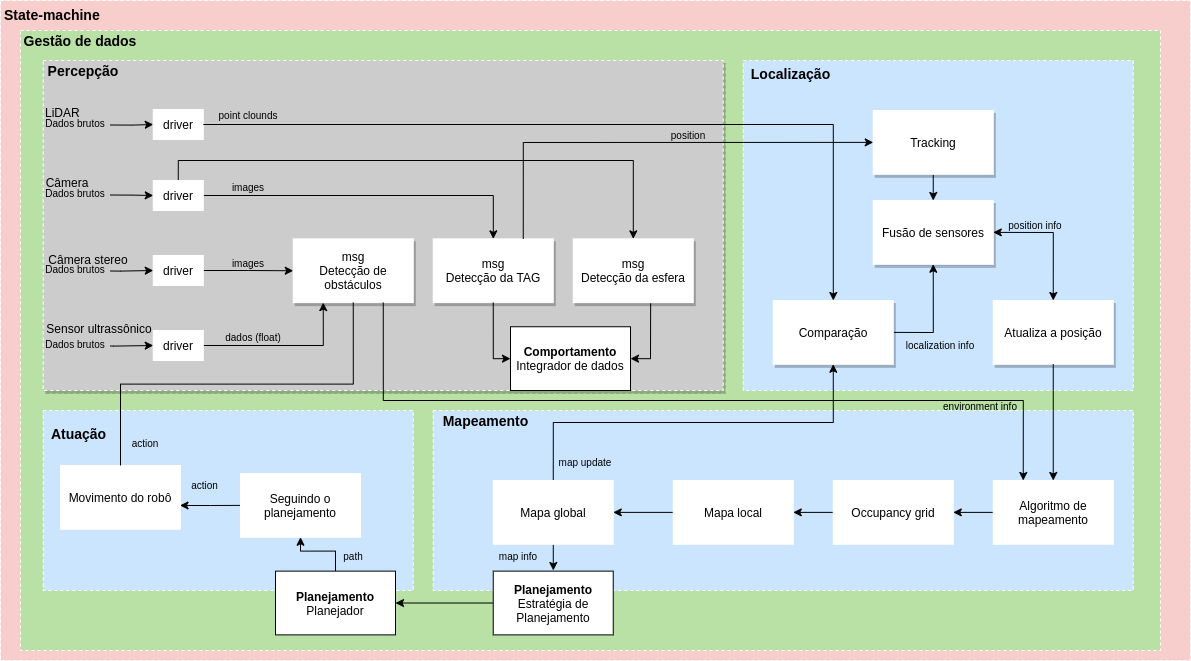
\includegraphics[width=0.75\textwidth]{diagrama_funcionalidades1.png}
        %\caption{.}
    \end{figure}
\end{frame}
%*----------- SLIDE (IMAGEM DO PROJETO) -------------------------------------------------------------
\begin{frame}[t]{Design}
    \framesubtitle{Funcionalidades}
    \begin{figure}
        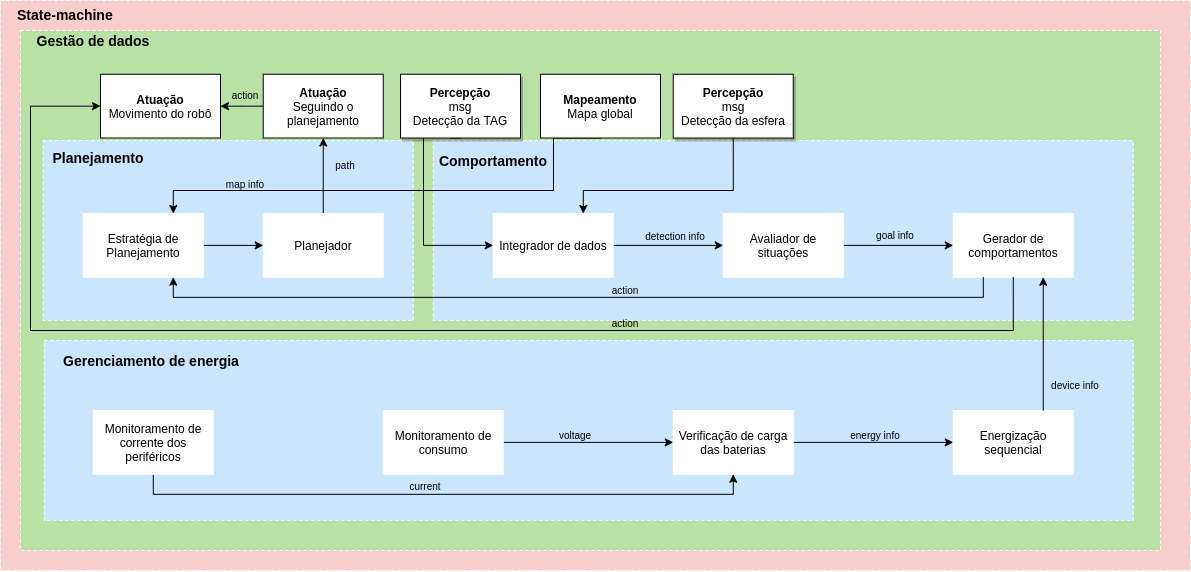
\includegraphics[width=0.8\textwidth]{diagrama_funcionalidades2.png}
        %\caption{.}
    \end{figure}
\end{frame}

%*----------- SLIDE (IMAGEM DO PROJETO) -------------------------------------------------------------
\begin{frame}[t]{Design}
    \framesubtitle{Estrutura analítica do projeto}
    \begin{figure}
        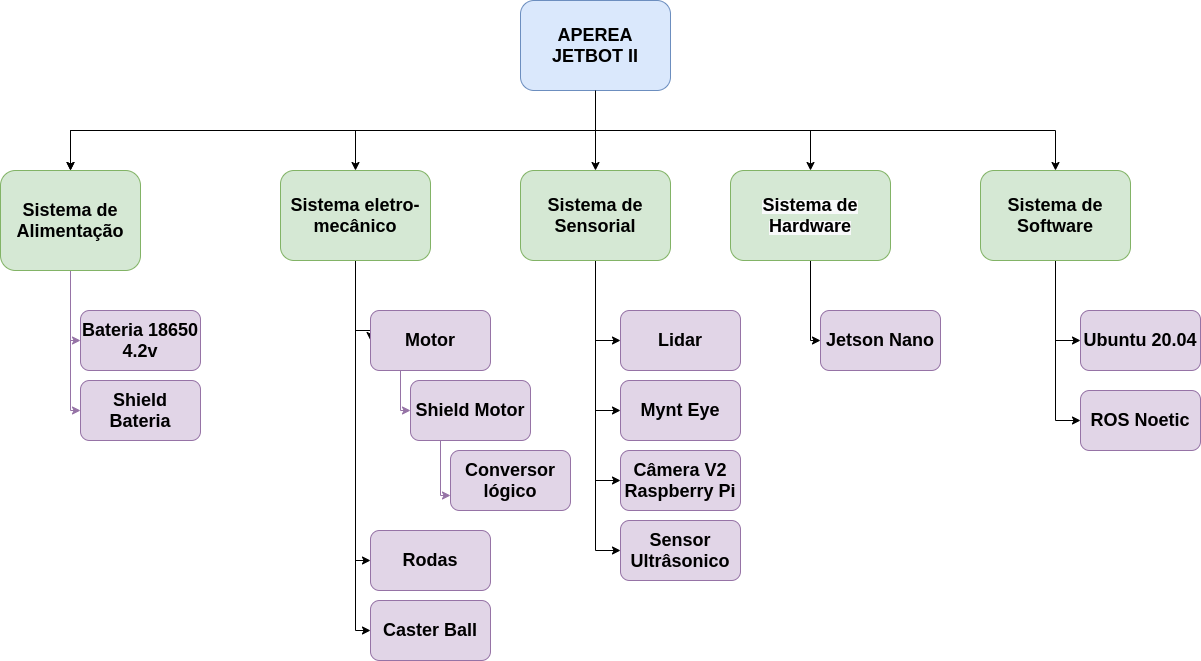
\includegraphics[width=0.75\textwidth]{PBS.png}
        %\caption{.}
    \end{figure}
\end{frame}